\documentclass[a4paper,12pt]{report}
\usepackage{titling}
\usepackage{graphics}
\usepackage{hyperref}
\usepackage{url}
\usepackage[italian]{babel}

\usepackage{listings}
\usepackage{color}
\usepackage{graphicx}
\usepackage{amsmath}
\usepackage{amssymb}
\usepackage{amsthm}
\usepackage{mathtools}
\usepackage{algorithm}
\usepackage{algpseudocode}
\usepackage{subcaption}
\usepackage{float}
\usepackage{multirow}
\usepackage{booktabs}
\usepackage{longtable}
\usepackage{array}
\usepackage{tabularx}
\usepackage{enumitem}
\usepackage{wrapfig}
\usepackage{lipsum}
\usepackage{titlesec}
\usepackage{multicol}
\usepackage{svg}
\usepackage{amsthm}
\usepackage[utf8]{inputenc}

\theoremstyle{definition}
\newtheorem{definition}{Definizione}[chapter]

\definecolor{mygreen}{rgb}{0,0.6,0}
\definecolor{mygray}{rgb}{0.5,0.5,0.5}
\definecolor{mymauve}{rgb}{0.58,0,0.82}

\begin{document}
\emergencystretch 3em
\begin{titlepage}
  \begin{center}
    \textbf{\LARGE Università della Calabria}\\
    \textbf{Dipartimento di Matematica e Informatica}\\
    \vskip 6pt
    \hrule
    \vskip 8pt
    
\includegraphics{res/logo.png}
    \vskip 8pt
    \textbf{Corso di Laurea Magistrale in Informatica}
    \vskip 32pt
    Tesi di Laurea

    \vskip 100pt
      { \large \bfseries GAEN: Generative AI for Enhanced Narrative - Rilevamento di Spoiler Mediante Modelli Generativi Avanzati}
    \vskip 170pt

    \noindent\begin{tabularx}{\textwidth}{@{}l @{\extracolsep{\fill}} r@{}}
      Relatori:       & Candidato:       \\ Prof.
      Gianluigi Greco & Alessandro Fazio \\ Prof.
      Kazumi Saito    & Matricola 242422 \\
    \end{tabularx}

    \vfill
    \hrule
    Anno Accademico 2024/2025
  \end{center}

\end{titlepage}

\newenvironment{dedication}
{\clearpage           % we want a new page
  \thispagestyle{empty}% no header and footer
  \vspace*{\stretch{1}}% some space at the top 
  \itshape             % the text is in italics
  \raggedleft          % flush to the right margin
}
{\par % end the paragraph
  \vspace{\stretch{3}} % space at bottom is three times that at the top
  \clearpage           % finish off the page
}

\begin{dedication}
  % I can't save you. Only you can save yourself.
\end{dedication}

\tableofcontents

\chapter{Introduzione}
\label{ch:introduzione}

\section{Contesto}
\label{sec:contesto}
Nell'era digitale, l'accesso immediato a contenuti
multimediali ha trasformato radicalmente il modo in cui
fruiamo di film, serie TV, libri e videogiochi.
Tuttavia, questa abbondanza di informazioni porta con sé
una sfida: la crescente esposizione a spoiler.
Gli spoiler, rivelando anticipatamente elementi cruciali
della trama, possono compromettere l'esperienza di
fruizione, generando frustrazione e delusione negli utenti.

Il problema degli spoiler è particolarmente rilevante in
contesti online, dove le discussioni e le recensioni
proliferano su forum, social media e piattaforme di
streaming.
La mancanza di strumenti efficaci per il rilevamento
automatico di spoiler rende difficile per gli utenti
proteggersi da tali rivelazioni indesiderate.

Questo lavoro propone di esplorare l'utilizzo di Large
Language Models (LLM) per affrontare la sfida del
rilevamento di spoiler.
L'obiettivo è sviluppare un sistema in grado di
identificare automaticamente gli spoiler in testi di varia
natura, sfruttando le capacità di comprensione del
linguaggio naturale degli LLM.

\section{Motivazioni}
\label{sec:motivazioni}
La motivazione principale di questa ricerca risiede nella
volontà di contribuire allo sviluppo di strumenti che
migliorino l'esperienza di fruizione di discussioni
riguardanti contenuti multimediali.
A tale scopo, è stato realizzato un sistema di rilevamento
di spoiler integrato in una estensione per browser, che
offre agli utenti un controllo maggiore sulla propria
esposizione a possibili spoiler.

Questo lavoro intende esplorare il potenziale degli LLM in
un'applicazione pratica e rilevante, provando a contribuire
alla comprensione delle loro capacità e limitazioni nel
contesto del rilevamento di informazioni specifiche in
testi complessi.

\section{Obiettivi}
\label{sec:obiettivi}

Gli obiettivi di questo lavoro sono i seguenti:

\begin{itemize}
      \item Realizzare un sistema di rilevamento di spoiler
            basato su Large Language Models.
      \item Valutare l'efficacia del sistema sviluppato nel
            rilevamento di spoiler in testi di varia natura.
      \item Integrare il sistema in un'estensione per browser
            e valutarne l'utilità e l'usabilità.
\end{itemize}

\section{Struttura del documento}
\label{sec:struttura-tesi}

Il resto del documento è organizzato come segue:

\begin{itemize}
      \item Nel Capitolo~\ref{ch:background} vengono
            presentati i concetti e le tecnologie alla base
            della ricerca, con particolare attenzione agli approcci
            possibili.
      \item Nel Capitolo~\ref{ch:lavori-correlati} vengono
            esaminati i lavori correlati, con un focus sulle
            ricerche relative al rilevamento di spoiler.
      \item Nel Capitolo~\ref{ch:sistema} viene descritta
            l'architettura del sistema di rilevamento di spoiler
            sviluppato, con particolare attenzione alla
            progettazione e alle scelte che hanno guidato lo sviluppo.
      \item Nel Capitolo~\ref{ch:valutazione} vengono
            presentati i risultati dell'analisi sperimentale
            condotta per valutare l'efficacia del sistema.
      \item Nel Capitolo~\ref{ch:owari} vengono
            riassunti i risultati ottenuti e vengono discusse
            le possibili direzioni future di ricerca.
\end{itemize}


\chapter{Background}
\label{ch:background}

\section{Approcci al problema}
\label{sec:approcci}

Di seguito vengono presentati alcuni approcci al problema
di rilevazione di spoiler in un testo.

\subsection{Approccio basato su regole}
\label{subsec:approccio-regole}

Un approccio molto semplice consiste nell'identificare
alcune parole chiave che sono tipicamente presenti in un
testo che contiene spoiler.
Ad esempio, le parole ``spoiler'' e ``spoiler alert'' sono
spesso utilizzate per avvertire il lettore che il testo
successivo contiene informazioni che potrebbero rovinare la
visione di un film o la lettura di un libro.
Altri esempi di parole chiave potrebbero essere i nomi di
personaggi o luoghi chiave della trama.
Questo approccio è molto semplice e può essere implementato
con poche righe di codice, ma ha il difetto di essere molto
limitato e di non essere in grado di rilevare spoiler più
sottili o nascosti.

Questo approccio è inoltre soggetto a molti falsi positivi,
ovvero a casi in cui il testo viene erroneamente
classificato come contenente spoiler quando in realtà non
lo contiene.
Ad esempio, una recensione di un film potrebbe contenere il
nome di un personaggio chiave della trama senza rivelare
informazioni cruciali sulla storia.
In questo caso, il testo non dovrebbe essere classificato
come contenente spoiler, ma l'approccio basato su regole
potrebbe erroneamente classificarlo come contenente
spoiler.

Oltre ai falsi positivi, questo approccio è anche soggetto
a falsi negativi, ovvero a casi in cui il testo contiene
spoiler ma non viene classificato come tale.
Ad esempio, una recensione di un film potrebbe contenere
informazioni cruciali sulla trama senza utilizzare le
parole chiave tipicamente associate agli spoiler, o in casi
anche più semplificati, potrebbe essere scritta in una
lingua diversa da quella in cui sono state definite le
parole chiave o contenere errori di battitura e di
ortografia che impediscono al sistema di riconoscere le
parole chiave.

Per questi motivi, l'approccio basato su regole non
promette risultati soddisfacenti e si è deciso di non
adottarlo in questo lavoro.

\subsection{Approccio basato su machine learning}
\label{subsec:approccio-ml}

Un approccio più sofisticato e promettente è quello basato
sul machine learning.
In questo approccio, si addestra un modello di machine
learning su un insieme di dati di addestramento
etichettati, ovvero un insieme di testi già classificati
come contenenti spoiler o non contenenti spoiler.
Il modello di machine learning impara a riconoscere i
pattern nei dati di addestramento e a classificare i testi
in base a tali pattern.
Una volta addestrato, il modello può essere utilizzato per
classificare nuovi testi come contenenti spoiler o non
contenenti spoiler.

Questo approccio ha il vantaggio di essere molto più
flessibile e potente rispetto all'approccio basato su
regole, in quanto il modello di machine learning è in grado
di riconoscere pattern complessi e sottili nei dati e di
generalizzare tali pattern ai nuovi dati.
Inoltre, il modello di machine learning è in grado di
adattarsi autonomamente ai nuovi dati, senza la necessità
di modificare manualmente le regole o i parametri del
sistema.

Tuttavia, l'approccio basato su machine learning ha anche
alcuni svantaggi.
In primo luogo, richiede un insieme di dati di
addestramento etichettati, che possono essere costosi e
laboriosi da ottenere a seconda del dominio di
applicazione.

Il secondo svantaggio è che il modello di machine learning
è difficile da realizzare e richiede competenze avanzate
per la sua implementazione.
Inoltre, il modello deve essere addestrato su un insieme di
dati di addestramento rappresentativo e bilanciato,
altrimenti potrebbe essere soggetto a overfitting o a
underfitting.

Generalizzando, l'approccio basato su machine learning è
più complesso e richiede più risorse rispetto all'approccio
basato su regole, ma promette risultati migliori e più
accurati.

\section{Approccio proposto}
\label{sec:approccio-proposto}

Per affrontare il problema della rilevazione di spoiler in
un testo, si propone di utilizzare un approccio basato su
machine learning.

L'intuizione alla base di questo approccio è che i LLM
(Large Language Model) sono in grado di catturare le
relazioni semantiche e sintattiche tra le parole e i
concetti all'interno di un testo, e quindi di riconoscere i
pattern che caratterizzano i testi contenenti spoiler.

In particolare, si propone di utilizzare un modello di LLM
pre-addestrato con lo scopo di \textbf{estrarre} lo spoiler da un
testo piuttosto che classificare l'intero testo come
contenente spoiler o non contenente spoiler, nel caso in
cui il testo contenga spoiler.

Utilizzare un modello di LLM pre-addestrato ha il vantaggio
di non richiedere un insieme di dati di addestramento
etichettati, in quanto il modello è già stato addestrato su
un vasto insieme di dati e ha imparato a riconoscere i
pattern nei testi in modo automatico e generale.

A prescindere dal modello di LLM utilizzato, si propone di
utilizzare un approccio basato su \textbf{RAG} (\textit{Retrieval-Augmented
Generation}) per arricchire il testo con informazioni
realitive al contesto in cui è stato scritto.
Ciò dovrebbe migliorare la qualità delle predizioni del
modello di LLM, in quanto il contesto può influenzare il
significato delle parole e dei concetti all'interno del
testo.

La difficolta principale di questo approccio è che i
modelli di LLM sono molto complessi e richiedono risorse
computazionali e di memoria considerevoli per essere
addestrati e utilizzati.
Inoltre, i modelli di LLM sono soggetti a fenomeni di
allucinazione e di bias, che possono influenzare le
predizioni del modello e ridurne l'accuratezza.

Tuttavia, nonostante queste difficoltà, gli LLM si sono
dimostrati molto efficaci in una varietà di task di NLP
(Natural Language Processing) e promettono risultati
soddisfacenti per il problema della rilevazione di spoiler
in un testo.

I dettagli dell'approccio proposto verranno discussi nei
seguenti capitoli.

\chapter{Lavori correlati}
\label{ch:lavori-correlati}

\section{Contesto della Ricerca}
\label{sec:contesto-della-ricerca}
In questo capitolo verranno presentati alcuni lavori
correlati all'oggetto di questo lavoro.
In particolare saranno introdotti alcuni concetti chiave e
verranno discussi in modo da poter contestualizzare meglio
il lavoro svolto.

\section{LLM, modelli di linguaggio}
\label{sec:llm-modelli-di-linguaggio}
I Large Language Models (LLM) rappresentano una classe di
modelli di deep learning che hanno dimostrato capacità
straordinarie nel comprendere e generare testo in
linguaggio naturale.
Questi modelli sono addestrati su enormi quantità di dati
testuali e sono in grado di apprendere complesse relazioni
semantiche e sintattiche tra le parole.

Nel contesto del rilevamento di spoiler, gli LLM offrono un
potenziale significativo grazie alla loro capacità di
comprendere il contesto e il significato delle parole.
A differenza dei modelli basati su regole o su approcci di
machine learning tradizionali, gli LLM potrebbero catturare
sfumature semantiche e identificare spoiler anche in testi
complessi e ambigui.

I primi modelli di LLM utilizzavano una architettura del
tipo \textit{encoder-decoder} per generare testo in
linguaggio naturale.
L'encoder è responsabile di trasformare il testo in input
in una rappresentazione vettoriale, mentre il decoder è
responsabile di generare il testo in output.

Con l'introduzione del \textbf{meccanismo di attenzione}, i
modelli LLM sono diventati sempre più potenti e
sofisticati.
Il meccanismo di attenzione permette al modello di estrarre
il contesto delle parole nel testo, migliorando
notevolemente le performance in una varietà di task.

L'attenzione è stata successivamente estesa a modelli
\textit{attention-based}, come il Transformer.

\subsection{Attention is all you need}
\label{sec:attention-is-all-you-need}
Il Transformer è un modello di deep learning
\textit{attention-based} introdotto da Vaswani et al.
nel 2017 nel paper ``Attention is
all you need''\cite{vaswani2017attention}.
Il Transformer ha rivoluzionato il campo del deep learning
per il linguaggio naturale, superando i modelli
\textit{encoder-decoder} in termini di performance e
efficienza \cite{google2017transformer}.

Il meccanismo di attenzione è il cuore del Transformer.
Questo meccanismo permette al modello di assegnare pesi
diversi alle parole nel testo in input, in modo da poter
focalizzare l'attenzione sulle parole più rilevanti per il
testo in input.

\begin{figure}[H]
  \centering
  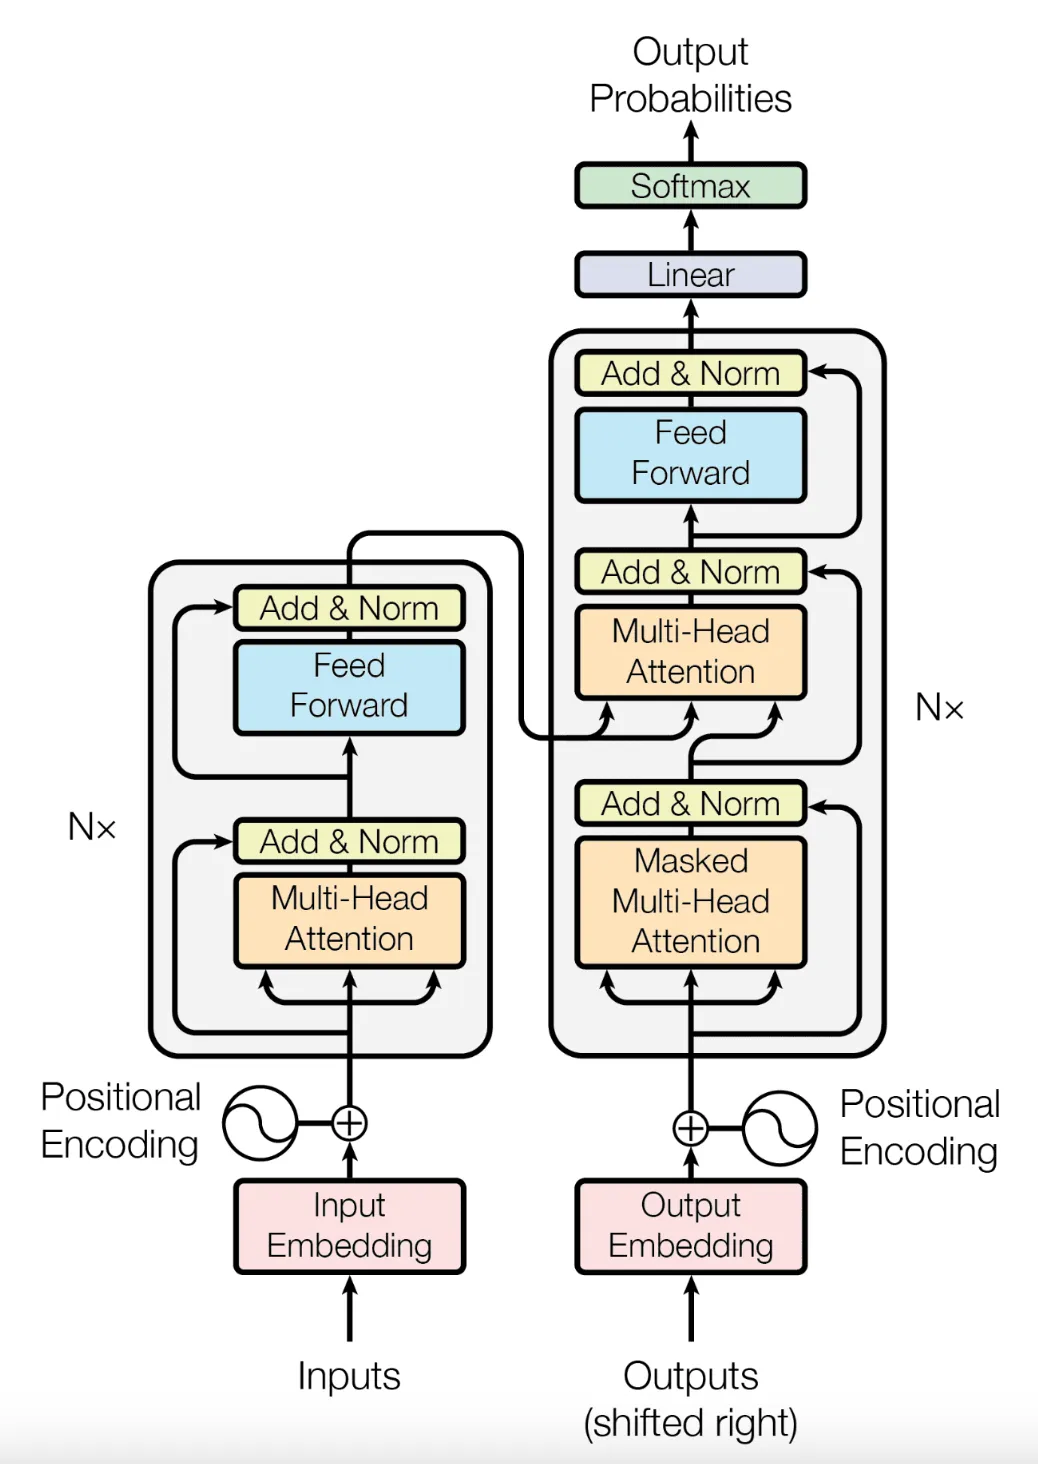
\includegraphics[width=0.6\textwidth]{res/transformer.png}
  \caption{Architettura del Transformer}
  \label{fig:transformer-architecture}
\end{figure}

\section{Embedding}
\label{sec:embedding}
Gli embedding sono una rappresentazione vettoriale di un
oggetto in uno spazio vettoriale.
Sono ampiamente utilizzati nel campo del deep learning per
rappresentare parole, frasi, documenti e immagini in modo
da poter essere usati come input per modelli di machine
learning \cite{mikolov2013efficient}.
Gli embedding vengono creati utilizzando modelli che
imparano a \textit{mappare} gli oggetti in uno spazio
vettoriale in modo che oggetti simili siano vicini tra
loro.
Tra i modelli di embedding più comuni troviamo
\textbf{Word2Vec}, \textbf{GloVe} e \textbf{FastText}.

Alcune delle applicazioni per gli embedding includono:

\begin{itemize}
  \item \textbf{Elaborazione del linguaggio naturale}: embedding
        di parole e frasi per modelli di classificazione,
        clustering e generazione di testo.
        Consentono al modello di comprendere il significato delle
        parole.
  \item \textbf{Sistemi di raccomandazione}: utilizzare gli
        embedding per rappresentare utenti, prodotti, post in uno
        spazio vettoriale, in modo da poterne calcolare la similarità.
  \item \textbf{Ricerca di immagini}: permettono di comparare
        immagini tra di loro o di comparare immagini e testo.
        Questo permette di cercare immagini tramite testo o
        viceversa.
  \item \textbf{Ricerca semantica}: rendono possibile la ricerca di
        frasi o documenti simili in base al loro significato.
\end{itemize}

Eseguire operazioni su embedding è molto più efficiente se
vengono memorizzati in un database apposito.

\begin{figure}[H]
  \centering
  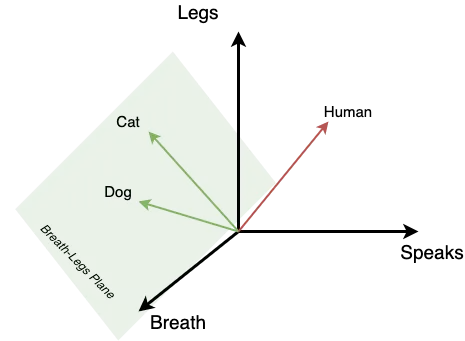
\includegraphics[width=0.5\textwidth]{res/embedding_space.png}
  \caption{Esempio di embedding. Fonte: \cite{olegborisovembeddingspace}}
  \label{fig:embedding-example}
\end{figure}

\subsection{Vector Database}
\label{sec:vector-database}
A differenza dei database tradizionali, i vector database
sono progettati per memorizzare e interrogare dati in forma
vettoriale.
Questo permette di effettuare operazioni e manipolazioni su
dati vettoriali in maniera più efficiente rispetto ad un
database relazionale.

I vector database sono particolarmente utili per
applicazioni che richiedono il calcolo della similarità tra
oggetti in uno spazio vettoriale, come le applicazioni
menzionate in precedenza.

Recentemente sono stati introdotti diversi vector database
come \textbf{Pinecone}, \textbf{Chroma} e \textbf{MongoDB
  Atlas}, ma per questo lavoro è stato scelto
\textbf{PostgreSQL} con il modulo \textit{PGVector} per
semplicità di utilizzo e familiarità.

\section{Fine-tuning di modelli}
\label{sec:finetuning-di-modelli}

Il finetuning è una tecnica comune nel campo del deep
learning per adattare un modello ad un task specifico.

Nel contesto del rilevamento di spoiler, il finetuning di
un modello può essere utile per migliorare le performance
del modello nel rilevare spoiler in un determinato contesto
o linguaggio.

Il finetuning di un modello pre addestrato comporta
l'addestramento del modello su un dataset specifico per un
numero limitato di epoche.
Questa tecnica consente di sfruttare le conoscenze
pregresse del modello, evitando di investire tempo e
risorse per addestrare un nuovo modello da zero.

Durante il finetuning, i pesi del modello vengono
aggiornati utilizzando un tasso di apprendimento più basso
rispetto all'addestramento iniziale.
Questo permette al modello di adattarsi al nuovo dataset
senza peggiorare le prestazioni su dati già visti.

Ciò risulta particolarmente utile quando si dispone di un
dataset limitato o quando si desidera adattare un modello
pre-addestrato a un dominio specifico.

\newpage
\section{Transizione all'implementazione}
\label{sec:transizione-implementazione}
Avendo stabilito il contesto teorico e tecnologico nel
capitolo corrente, il prossimo passo consiste nel
descrivere come questi concetti sono stati applicati nella
pratica.
Nel prossimo capitolo ci focalizzeremo sugli aspetti
pratici della realizzazione del sistema.
Descrivendo in dettaglio il design e l'implementazione del
sistema di rilevamento di spoiler, illustrando le sfide
incontrate e le soluzioni adottate per creare
un sistema efficace e utilizzabile.

\chapter{Design e implementazione}
\label{ch:sistema}

\section{Introduzione}
Inizieremo con una panoramica generale dell'architettura
del sistema, per poi passare a una descrizione dettagliata
dei componenti principali.

\section{Architettura del sistema}
\label{sec:architettura}
L'architettura del sistema è composta dalle seguenti componenti principali:

\begin{itemize}
      \item \textbf{Frontend}: consiste in una estensione per il browser che
            permette di interagire con il sistema.
      \item \textbf{Backend}: è il server che gestisce le richieste
            provenienti dal frontend e comunica con il database e il LLM.
      \item \textbf{Embedder}: è il componente che genera gli embedding
            delle parole chiave che popolano il database, nonchè gli embedding
            delle richieste del frontend.
      \item \textbf{Database}: memorizza le informazioni relative agli embedding
            delle parole chiave che fungono da input al LLM.
      \item \textbf{LLM}: è il modello che genera le risposte in base
            alle richieste del frontend.
\end{itemize}

\begin{figure}
      \centering
      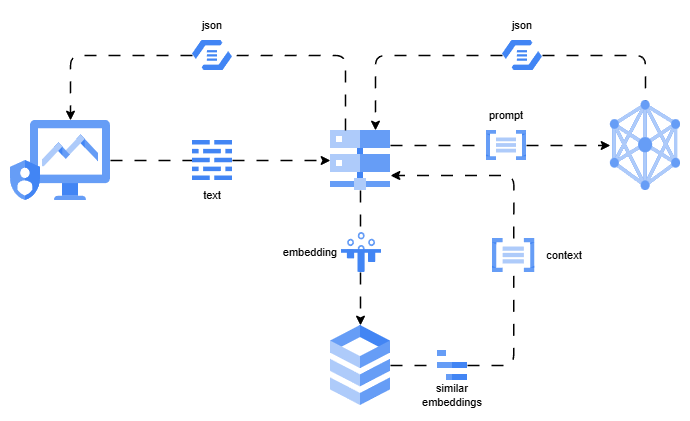
\includegraphics[width=1\textwidth]{res/architecture.png}
      \caption{Architettura del sistema e flusso dei dati}
      \label{fig:architettura}
\end{figure}

\section{Componenti principali}
\label{sec:componenti}
\subsection{Frontend}
\label{sec:frontend}
Il frontend è un'estensione per il browser che consente di
interagire con una qualsiasi pagina web.
L'estensione è progettata per essere leggera e veloce, in
modo da non influire sulle prestazioni del browser.

Il frontend è responsabile della raccolta delle
informazioni, oltre che della visualizzazione dei
risultati.
Quando l'utente seleziona un elemento della pagina, il
frontend estrae il contenuto testuale e lo invia al backend
per l'elaborazione.
Il backend genera quindi una risposta e la invia al
frontend, che la visualizza all'utente.

Inoltre, il frontend permette di selezionare quale modello
utilizzare per generare le risposte, in modo da poter
testare le prestazioni di diversi modelli.

\subsection{Backend}
\label{sec:backend}

Il backend è il cuore del sistema, responsabile della
gestione delle richieste provenienti dal frontend e della
comunicazione con il database e il LLM.
Il backend è implementato in Python e utilizza il framework
FastAPI che permette la creazione di API RESTful, per
applicazioni web scalabili e performanti.
Il backend è progettato per essere modulare e facilmente
estensibile, in modo da poter aggiungere nuove funzionalità
in futuro.

Quando il backend riceve una richiesta dal frontend, esegue
le seguenti operazioni:
\begin{itemize}
      \item Preprocessa il contenuto testuale dalla richiesta
      \item Tokenizza il testo dividendo il testo in frasi
            più piccole.\\
            \textbf{Questo passaggio è fondamentale per creare il contesto
                  necessario per il LLM.}
      \item Genera gli embedding di ogni frase attraverso
            l'embedder.
      \item Esegue una ricerca nel database per trovare le
            parole chiave più simili agli embedding generati
      \item Invia la richiesta al LLM per generare la risposta.
            La richiesta al LLM include il contenuto processato e le
            parole chiave trovate nel database.
      \item Restituisce la risposta del LLM al frontend sotto forma di
            JSON.
\end{itemize}

La comunicazione tra il server e il LLM avviene tramite la
libreria di OpenAI, che consente di inviare richieste al
modello e ricevere le risposte utilizzando una interfaccia
configurabile.
In particolare, la libreria permette di utilizzare qualiasi
modello compatibile con l'interfaccia di OpenAI e questo ha
permesso di testare diversi modelli attraverso il tool
\textbf{Ollama}.

\subsection{Ollama}
\label{sec:ollama}
Ollama è un tool open source che consente di eseguire LLM
localmente, senza la necessità di una connessione a
Internet.
Ollama stato è progettato per essere semplice da usare e
consente di eseguire modelli LLM in modo rapido e
efficiente sfruttando l'accelerazione hardware delle GPU
quando possibile.
Ollama offre una varieta di modelli LLM pre-addestrati, tra
cui \texttt{Llama}, \texttt{Mistral}, \texttt{Phi},
\texttt{Deepseek} e \texttt{Gemma}.

In particolare, \texttt{Gemma} è il modello utilizzato per
testare il sistema, in quanto è ottimizzato per l'uso in
locale e offre prestazioni eccellenti rispetto a modelli di
dimensioni comparabili.

\subsection{Embedder}
\label{sec:embedder}
L'embedder è il componente responsabile della generazione
degli embedding delle parole chiave che popolano il
database, nonchè degli embedding delle richieste del
frontend.
L'embedder è implementato in Python e utilizza la libreria
\texttt{SentenceTransformers}\cite{reimers-2019-sentence-bert}
per generare gli embedding delle parole chiave e delle
richieste.

Attraverso l'uso di \texttt{SentenceTransformers} è stato
possibile eseguire il fine-tuning del modello di embedding
\texttt{all-MiniLM-L6-v2} per ottimizzare le prestazioni
del sistema.
Il fine-tuning del modello è stato eseguito utilizzando un
dataset autonomamente creato, tramite l'uso di un web
scraper che ha estratto le informazioni da fonti pubbliche
disponibili su Internet.

Il dataset è composto da una serie di articoli e documenti
che sono stati manipolati per estrarre il contenuto
testuale e le parole chiave.

\section{Dataset e tool utilizzati}
\label{sec:dataset}

Qui di seguito sono riportati i tool e le librerie
utilizzati per la creazione del dataset e il fine-tuning
del modello di embedding:

\begin{itemize}
      \item \textbf{Puppeteer}: è una libreria Node.js che consente di
            controllare un browser Chrome o Chromium in modo
            programmatico.
      \item \textbf{Pandas}: è una libreria Python per la manipolazione e
            l'analisi dei dati.
      \item \textbf{Visualizer}: un tool creato appositamente per
            visualizzare i risultati dello scraping, utilizzato per
            verificare la correttezza dei dati estratti e studiare le
            relazioni tra le parole chiave e i documenti.
\end{itemize}

\begin{figure}[H]
      \centering
      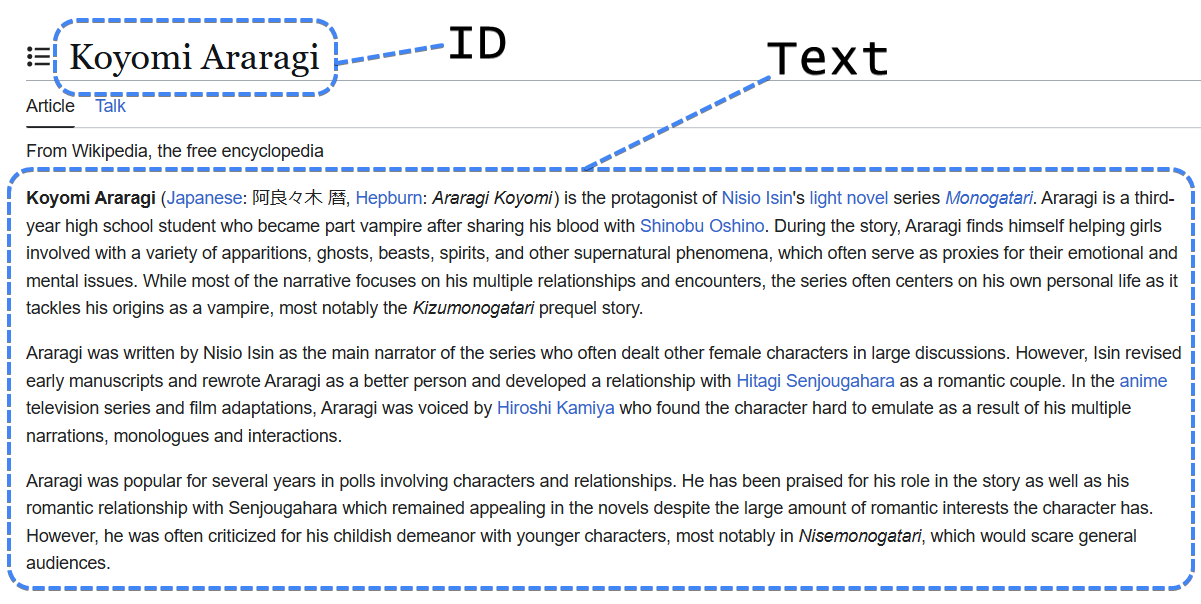
\includegraphics[width=0.8\textwidth]{res/scraper.png}
      \caption{fonte: Wikipedia}
      \label{fig:visualizer}
\end{figure}

In figura \ref{fig:visualizer} è mostrato un esempio di
scraping effettuato attraverso il tool, che ha estratto il
contenuto testuale di una pagina Wikipedia.

Notiamo che il tool è in grado di estrarre non solo il
contenuto testuale, ma anche i collegamenti ad altre pagine
presenti nei singoli paragrafi, unitamente a una serie di
metadati.
Ciò ha reso possibile la creazione di un grafo delle
relazioni tra le parole chiave e i documenti, che è stato
utilizzato per il fine-tuning del modello di embedding.
Il grafo è stato creato utilizzando la libreria
\texttt{D3.js}, che consente di creare visualizzazioni
interattive dei dati.

\subsection{Visualizer}
\label{sec:visualizer}
Il visualizer è stato creato appositamente per studiare le
relazioni tra le parole chiave e i documenti, in modo da
ottimizzare il fine-tuning del modello di embedding creando
un dataset bilanciato e di qualità superiore.

\begin{figure}[H]
      \centering
      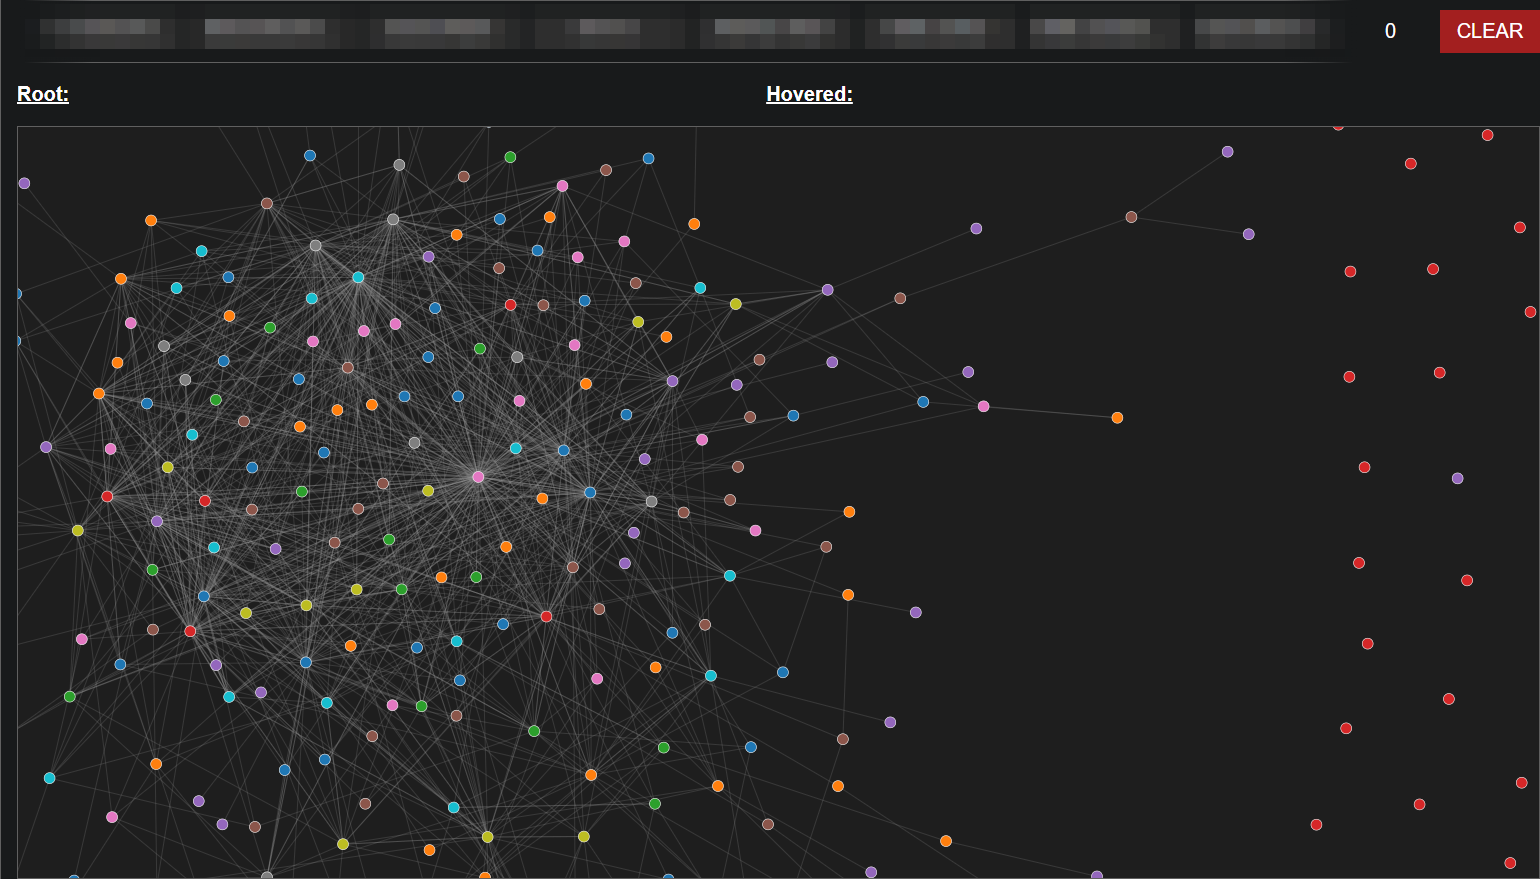
\includegraphics[width=0.8\textwidth]{res/vis1.png}
      \caption{Esempio di grafo creato dal visualizer}
      \label{fig:vis1}
\end{figure}

In figura \ref{fig:vis1} è mostrato un esempio di grafo.
Ogni nodo rappresenta un documento e ogni arco rappresenta
una relazione tra due documenti.

Possiamo osservare che alcuni documenti sono più connessi
di altri, il che indica che hanno diversi collegamenti, o
che diversi documenti fanno riferimento a loro.
E' anche possibile osservare che alcuni documenti sono
isolati, il che indica che non hanno collegamenti con altri
documenti.

Attraverso il visualizer è stato possibile filtrare i
documenti in base a diversi criteri, come ad esempio il
numero di collegamenti, metadati, o altri tipi di filtro.

Nella scelta dei documenti da includere nel dataset si è tenuto
conto di diversi fattori statistici \cite{Newman2010}
\cite{Newman2002Assortative} \cite{Newman2003Mixing},
elencati di seguito:

\begin{table}[htbp]
      \centering
      \caption{Statistiche globali del grafo}
      \label{tab:graph_stats}
      \begin{tabularx}{\textwidth}{@{}l @{\extracolsep{\fill}} r@{}}
            \toprule
            Statistica                           & Valore  \\
            \midrule
            Coefficiente di assortatività        & -0.4677 \\
            Mescolanza di assortatività discreta & -0.0059 \\
            Diametro del grafo                   & 9       \\
            Densità del grafo                    & 0.024   \\
            Lunghezza media del percorso         & 3.85    \\
            Nodi isolati                         & 76      \\
            \bottomrule
      \end{tabularx}
\end{table}

\begin{table}[H]
      \centering
      \caption{Statistiche per singoli nodi}
      \label{tab:node_stats}
      \begin{tabularx}{\textwidth}{@{}l @{\extracolsep{\fill}} r@{}}
            \toprule
            Statistica                 & Valore \\
            \midrule
            Coefficiente di Clustering & 0.333  \\
            Componenti nel Cluster     & 258    \\
            Centralità di Closeness    & 0.365  \\
            \bottomrule
      \end{tabularx}
\end{table}

\noindent
\textbf{Nota:}
I valori riportati nelle tabelle \ref{tab:graph_stats} e
\ref{tab:node_stats} sono stati generati su un dataset di
esempio per illustrare le funzionalità del visualizer.

\section{Preparazione del dataset}
\label{sec:dataset_prep}
Per preparare il dataset è stato necessario eseguire
diverse operazioni di post-processing sui dati estratti
dallo scraping.

In particolare, sono stati eseguiti i seguenti passaggi:
\begin{itemize}
      \item Rimozione dei metadati
      \item Normalizzazione del testo
      \item Oversampling di alcune parole chiave
      \item Introduzione di rumore nel dataset
      \item altre operazioni (ulteriori dettagli sono
            disponibili nel codice sorgente)
\end{itemize}

Si è deciso di eseguire l'oversampling di alcuni tipi di
parole chiave, in modo da bilanciare il dataset e ottenere
un modello di embedding più robusto.

Un esempio di oversampling è mostrato in figura
\ref{fig:oversampling}.

\begin{figure}[H]
      \centering
      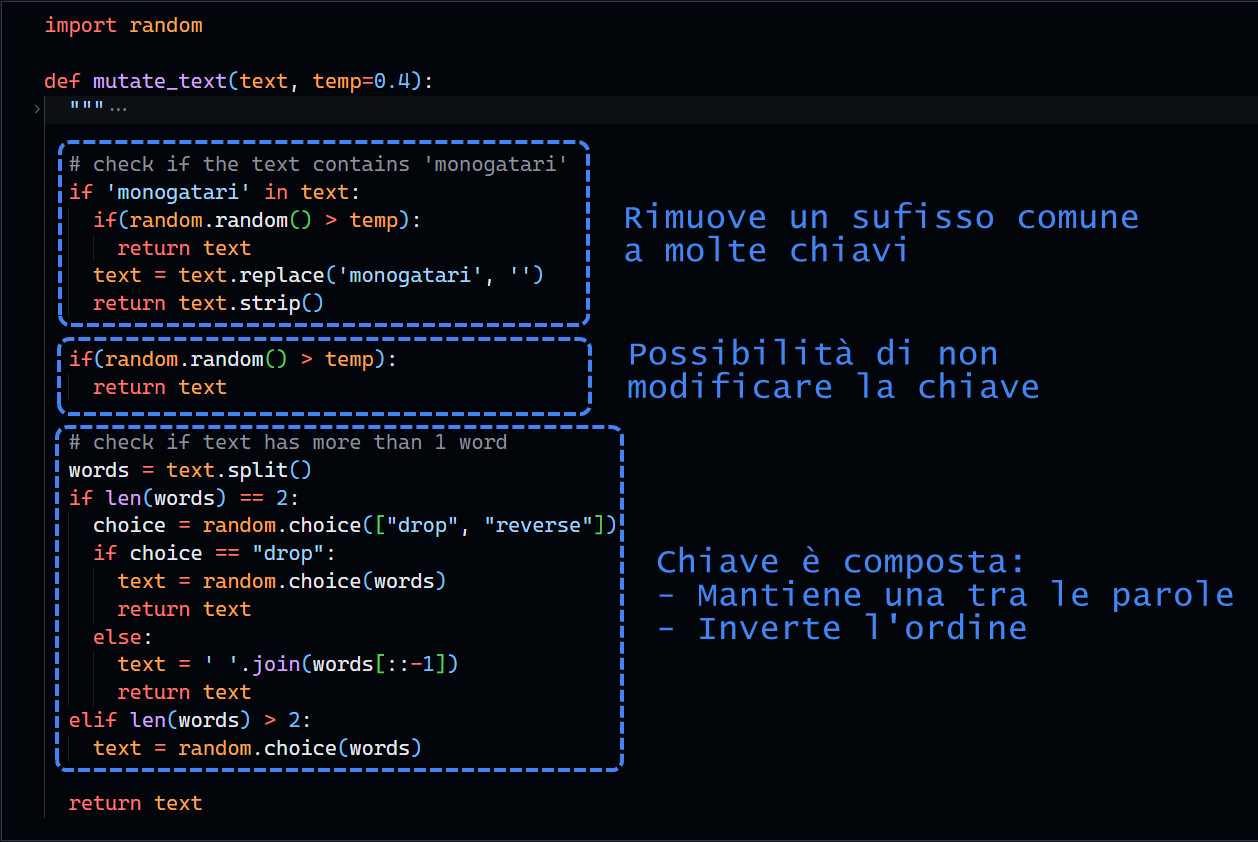
\includegraphics[width=0.6\textwidth]{res/noise.png}
      \caption{Esempio di oversampling}
      \label{fig:oversampling}
\end{figure}

Il risultato finale del dataset è stato un file JSON con il seguente formato:

\begin{table}[H]
      \centering
      \caption{Formato del dataset}
      \label{tab:dataset_format}
      \begin{tabularx}{\textwidth}{l@{\extracolsep{\fill}} l @{\extracolsep{\fill}}l}
            \toprule
            anchor         & positive                                                                                            & negative     \\
            \midrule
            koyomi araragi & vampiro, studente, adolescente                                                                      & nobile       \\
            shinobu oshino & vampiro, 500 anni, nobile                                                                           & studente     \\
            ononoki        & sissi, yay. peace peace! \faHandPeace[regular]\faEye[regular]\_\faEye[regular]\faHandPeace[regular] & hatsune miku \\
            bakemonogatari & anime, manga, light novel                                                                           & film         \\
            nise           & anime, manga, light novel                                                                           & film         \\
            \bottomrule
      \end{tabularx}
\end{table}

\noindent
\textbf{Nota:}
I dati riportati nella tabella \ref{tab:dataset_format}
sono stati generati su un dataset di esempio per illustrare
il formato del dataset.
\newline

In particolare, la colonna \texttt{anchor} contiene la
parola chiave, la colonna \texttt{positive} contiene il
contesto che si desidera associare all'ancora, mentre la
colonna \texttt{negative} contiene l'elemento che si
desidera evitare di associare alla parola chiave.

Tramite l'uso di questo formato è stato possibile separare
efficacemente le parole chiave e i contesti, in modo da
ottenere un dataset qualitativamente migliore.

\subsection{Scelta dei negativi}
\label{sec:negatives}
La scelta degli esempi negativi è stata cruciale per il
fine-tuning del modello di embedding.

Esistono principalmente due approcci per la scelta degli
esempi negativi:

\begin{itemize}
      \item \textbf{Scelta casuale}: consiste nel selezionare
            casualmente gli esempi negativi dal dataset.
      \item \textbf{Scelta non casuale}: consiste nel
            selezionare gli esempi negativi in base a regole
            stabilite.
\end{itemize}

Nel primo approccio, la scelta degli esempi negativi è
completamente casuale e non tiene conto delle relazioni tra
le parole chiave e i contesti.
Questo approccio può portare a risultati non ottimali, in
quanto gli esempi negativi potrebbero non essere
rappresentativi del contesto in cui si desidera utilizzare
il modello di embedding.

La strategia adottata nel progetto è stata quella di
estrarre randomicamente il contesto a partire dalle parole
chiave ``vicine" all'ancora di riferimento.
Questo approccio tiene conto delle relazioni tra i diversi
documenti in modo da ottenere degli embedding più robusti e
rappresentativi.

Nel nostro caso, a partire da un nodo del grafo, l'ancora è
rappresentata dal titolo del nodo, l'esempio positivo è
rappresentato dal contenuto del nodo, mentre l'esempio
negativo è rappresentato dal contenuto di un nodo
adiacente.

Questo approccio ha portato a risultati migliori rispetto
all'approccio casuale poichè sfrutta il fatto che i
documenti che hanno collegamenti in comune, molto
probabilmente condividono informazioni simili.
Permettendo al modello di distinguere tra i due, è stato
possibile ottenere un embedding più robusto e
rappresentativo.

\section{Fine-tuning del modello}
\label{sec:fine_tuning}
Il fine-tuning del modello di embedding è stato eseguito
utilizzando la libreria \texttt{SentenceTransformers} e il
dataset creato in precedenza.
Il fine-tuning è stato eseguito utilizzando il modello
\texttt{all-MiniLM-L6-v2}, che è un modello di embedding
pre-addestrato basato su \texttt{BERT} e ottimizzato per
l'uso in locale.
Il fine-tuning è stato eseguito utilizzando il dataset
creato in precedenza e il modello è stato addestrato per un
numero di epoche pari a 4.

La funzione di penalità utilizzata è stata la
\texttt{TripletLoss}\cite{hermans2017defense}, comunemente
utilizzata per l'addestramento di modelli di embedding.
La \texttt{TripletLoss} è progettata per minimizzare la
distanza tra l'ancora e l'esempio positivo, e massimizzare
la distanza tra l'ancora e l'esempio negativo.
\\

\noindent
Come discuteremo nel prossimo capitolo, il fine-tuning del
modello ha permesso di ottenere un modello di embedding
robusto e rappresentativo.

\chapter{Valutazione}
\label{ch:valutazione}

\section{Introduzione}
\label{sec:introduzione}
In questo capitolo, presentiamo i risultati ottenuti
durante la fase di valutazione del nostro sistema.

Inizieremo con una panoramica dei dati utilizzati per il
fine-tuning e la valutazione del modello, seguita da una
descrizione delle metriche di valutazione impiegate.

Successivamente, presenteremo i risultati ottenuti,
analizzando le prestazioni del nostro sistema in termini di
accuratezza e capacità di rilevamento degli spoiler.

Discuteremo le implicazioni dei risultati e le possibili
direzioni future per il miglioramento del sistema.

\subsection{Specifiche tecniche}
\label{sec:specs}
La configurazione del sistema è stata eseguita su un
computer con le seguenti specifiche:

\begin{itemize}
  \item CPU: AMD Ryzen 7 5800H (8 core, 16 thread)
  \item GPU: NVIDIA GeForce RTX 3070 Laptop (8 GB)
  \item RAM: 16 GB
  \item Sistema operativo: Windows 10 22H2
  \item Versione di Python: 3.12.9
\end{itemize}

\section{Dataset e metodologia}
\label{sec:dataset_eval}

Per la valutazione del nostro sistema, abbiamo utilizzato 2
strategie: \textbf{pair} e \textbf{triplet}.
Il dataset \textbf{pair} è derivato da \textbf{triplet}
escludendo la colonna \textit{negative}.
Questo ha permesso di valutare il sistema in diverse
configurazioni.

Il codice per la generazione degli split e il training è
identico per entrambe le strategie, con l'unica differenza
che per \textbf{pair} il dataset è stato ridotto a 2
colonne: \textit{positive} e \textit{negative}, adattando
la funzione di loss di conseguenza.
Il seed utilizzato per la generazione degli split è
298\cite{nisemonogatari_ep1}, garantendo la riproducibilità
dei risultati.

\begin{table}[H]
  \centering
  \begin{tabularx}{\textwidth}{l @{\extracolsep{\fill}} r}
    \toprule
    \textbf{Parametro} & \textbf{Valore}       \\
    \midrule
    Dataset            & 4067 righe            \\
    Split              & 80\% train, 20\% test \\
    Epoche             & 4                     \\
    Loss (pair)        & CosineSimilarityLoss  \\
    Loss (triplet)     & TripletLoss           \\
    \bottomrule
  \end{tabularx}
  \caption{Panoramica dei parametri utilizzati per il fine-tuning e la valutazione del modello.}
  \label{tab:dataset_eval}
\end{table}

\section{Embedders}
\label{sec:embedders_eval}
Durante la creazione del sistema, si è deciso di
utilizzare due modelli pre-addestrati per generare gli embedding:

\begin{itemize}
  \item \textbf{all-MiniLM-L6-v2}
  \item \textbf{all-mpnet-base-v2}
\end{itemize}

Nessuno dei modelli è stato addestrato su dati specifici al
dominio degli spoiler o sui dati utilizzati per il
fine-tuning.
Come mostrano i risultati di seguito, nessuno dei modelli
soddisfaceva i requisiti per il task dato il dominio
specifico, ma con un fine-tuning adeguato, sono stati in
grado di generare embeddings soddisfacenti.

Entrambi i modelli sono disponibili su HuggingFace,
installando la libreria \texttt{sentence-transformers}.
I modelli scelti sono comunemente utilizzati per la
creazione di embeddings per frasi o paragrafi brevi,
rendendoli adatti al nostro task.
Il codice per il fine-tuning e la valutazione è stato
scritto in Python ed è disponibile su GitHub.
% link github

\newpage
\subsection{Risultati}
\label{sec:risultati}
\textbf{Nota:} I migliori risultati sono segnalati con un asterisco
(\textbf{*})

\subsubsection{Pair}
\label{sec:pair}
\begin{table}[H]
  \centering
  \begin{tabularx}{\textwidth}{l @{\extracolsep{\fill}} r}
    \toprule
    Modello                     & {Similarità positiva} \\
    \midrule
    \multicolumn{2}{c}{\textbf{Pre-addestramento}}      \\
    \midrule
    all-mpnet-base-v2           & 0.1554                \\
    \textbf{all-MiniLM-L6-v2}*  & \textbf{0.1688}       \\
    \midrule
    \multicolumn{2}{c}{\textbf{Fine-tuned}}             \\
    \midrule
    \textbf{all-mpnet-base-v2}* & \textbf{0.9975}       \\
    all-MiniLM-L6-v2            & 0.9938                \\
    \bottomrule
  \end{tabularx}
  \caption{Risultati della valutazione dei modelli di embedding (Pair)}
  \label{tab:embedding_pair}
\end{table}

\subsubsection{Triplet}
\label{sec:triplet}
\begin{table}[H]
  \centering
  \begin{tabularx}{\textwidth}{l @{\extracolsep{\fill}} r @{\extracolsep{\fill}} r}
    \toprule
    Modello                     & {Similarità positiva} & {Similarità negativa} \\
    \midrule
    \multicolumn{3}{c}{\textbf{Pre-addestramento}}                              \\
    \midrule
    all-mpnet-base-v2           & 0.1554                & 0.2001                \\
    \textbf{all-MiniLM-L6-v2}*  & \textbf{0.1688}       & \textbf{0.2113}       \\
    \midrule
    \multicolumn{3}{c}{\textbf{Fine-tuned}}                                     \\
    \midrule
    \textbf{all-mpnet-base-v2}* & \textbf{0.6358}       & \textbf{-0.8118}      \\
    all-MiniLM-L6-v2            & 0.6274                & -0.7221               \\
    \bottomrule
  \end{tabularx}
  \caption{Risultati della valutazione dei modelli di embedding (Triplet)}
  \label{tab:embedding_triplet}
\end{table}

Notiamo che i risultati pre-addestramento sono molto bassi,
e simili tra loro, il che indica che i modelli non sanno
distinguere categorizzare bene i dati in input.
Tuttavia, dopo il fine-tuning, i risultati sono
significativamente migliorati, con all-mpnet-base-v2 che
ottiene i migliori risultati in entrambe le configurazioni.
Da notare che i risultati nella configurazione
\textbf{pair} sono migliori rispetto a quelli nella
configurazione \textbf{triplet}, ma ciò indica solo che i
modelli hanno appreso a generare embedding più simili tra
loro, \textbf{non necessariamente più accurati}.

\subsection{Considerazioni}
\label{sec:considerazioni}

In definitiva, i risultati mostrano che il fine-tuning ha
portato a un miglioramento significativo delle prestazioni,
specialmente nella configurazione \textbf{triplet}, dove i
modelli sono stati in grado di generare embedding con una
similarità positiva superiore a $0.64$ e una similarità
negativa inferiore a $-0.81$.
Ciò indica che i modelli sono stati in grado di raggruppare
correttamente i dati simili e separare quelli dissimili,
dimostrando la loro efficacia in questo task dopo un
adeguato fine-tuning.

Nononstante all-mpnet-base-v2 abbia ottenuto, di poco,
risultati migliori rispetto a all-MiniLM-L6-v2,
quest'ultimo ha dimostrato di essere più veloce e più
leggero, rendendolo la scelta preferita per questo
progetto.
Inoltre, all-MiniLM-L6-v2 ha mostrato prestazioni migliori
in fase di fine-tuning.

\subsection{Prestazioni in fase di fine-tuning}
\label{sec:prestazioni-fine-tuning}

\begin{table}[H]
  \centering
  \begin{tabularx}{\textwidth}{l @{\extracolsep{\fill}} c @{\extracolsep{\fill}} c @{\extracolsep{\fill}} r}
    \toprule
    Modello           & {Tempo (min:sec)} & Step & {Perdita} \\
    \midrule
    all-mpnet-base-v2 & 03:26             & 500  & 3.8035    \\
    all-MiniLM-L6-v2  & 00:53             & 500  & 4.0104    \\
    \bottomrule
  \end{tabularx}
  \caption{Tempi e perdite del fine-tuning (Triplets)}
  \label{tab:finetuning_triplets}
\end{table}

\begin{table}[H]
  \begin{tabularx}{\textwidth}{l @{\extracolsep{\fill}} c @{\extracolsep{\fill}} c @{\extracolsep{\fill}} r}
    \toprule
    Modello           & {Tempo (min:sec)} & Step & {Perdita} \\
    \midrule
    all-mpnet-base-v2 & 02:10             & 500  & 0.0183    \\
    all-MiniLM-L6-v2  & 00:37             & 500  & 0.0263    \\
    \bottomrule
  \end{tabularx}
  \caption{Tempi e perdite del fine-tuning (Pairs)}
  \label{tab:finetuning_pairs}
\end{table}

Le prestazioni di all-MiniLM-L6-v2 sono decisamente
migliori rispetto a quelle di all-mpnet-base-v2 in termini
di tempo.
Il tempo di inferenza è un aspetto critico per
l'implementazione di modelli che devono essere utilizzati
in locale, e questo modello ha dimostrato di essere la
scelta più adatta per il nostro scopo.

\section{LLM}
\label{sec:llm_eval}

Per la valutazione del modello LLM, è stato scelto
\textbf{Gemma3}.

\subsection{Gemma3}
\label{sec:gemma3}
Gemma3 è un modello LLM open-weight sviluppato da Google,
progettato per essere altamente efficiente e performante.
Gemma3 ha capacità multimodali, il che significa che può
elaborare testo e immagini.

Data la sua architettura avanzata derivante da Gemini, lo
stato dell'arte dei modelli di Google, Gemma3 è in grado di
comprendere e generare contenuti con performance
competitive rispetto a modelli di dimensioni molto
maggiori\cite{gemma_2025}.

Per questo progetto, non abbiamo utilizzato la modalità
multimodale, ma ci siamo concentrati sulla generazione di
testo.

Si è deciso di utilizzare Gemma3 per la sua capacità di
generare testo di alta qualità e la sua architettura
leggera che consente un'implementazione rapida ed
efficiente a latenza ridotta.

A causa di limitazioni hardware, non è stato possibile
scaricare il modello completo, quindi è stato scelto di
utilizzare versioni del modello con dimensioni diverse.
Gemma3 è disponibile in diverse dimensioni:

\begin{itemize}
  \item \textbf{Gemma3-1B}: 1 miliardo di parametri
  \item \textbf{Gemma3-4B}: 4 miliardi di parametri
  \item \textbf{Gemma3-12B}: 12 miliardi di parametri
  \item \textbf{Gemma3-27B}: 27 miliardi di parametri
\end{itemize}

La versione 1B non possiede la capacità multimodali, mentre
la versione 12B ha una dimensione $>8GB$, per cui non è
stato possibile utilizzare appieno il modello sfruttando
l'accelerazione GPU.
Per questo motivo, sono stati utilizzati principalmente i
modelli 1B e 4B.

\subsection{Risultati LLM}
\label{sec:llm_results}

Per valutare le prestazioni dei diversi LLM, è stato
utilizzato un dataset diverso rispetto a quello utilizzato
per il fine-tuning e la valutazione del modello di
embedding.

Il dataset è composto da 100 frasi, ognuna delle quali è
stata generata da un utente diverso.
Le frasi possono contenere spoiler o meno, e in caso di
spoiler, viene marcato l'estratto che contiene lo spoiler.

Il dataset è stato procurato tramite scraping del sito
\textbf{TVTropes}, un sito dedicato alla discussione di
opere di narrativa e alla loro analisi.

Il dataset è stato bilanciato in modo da avere un numero
uguale di frasi con e senza spoiler.
Le frasi sono state estratte in modo casuale dalla comunità
dedicata all'opera \textbf{Monogatari Series}, che è anche
l'oggetto del dataset utilizzato per il fine-tuning del
modello di embedding.

Si è scelto di mantenere il preprocessamento del dataset al
minimo, poiché le frasi sono state raccolte direttamente
dal sito web.
Questo approccio permette di preservare la qualità naturale
del linguaggio utilizzato dagli utenti reali.
Il dataset risultante rappresenta un campione autentico di
espressioni, caratterizzato da varietà di stili e
dall'assenza di schemi predefiniti.

Questa eterogeneità pone una sfida significativa per il
modello, che non è stato addestrato su dati di questa
natura e si trova ad affrontare un tipo di input inedito.

La Tabella \ref{tab:risultati-llm} riassume i risultati
ottenuti dai vari modelli.

\begin{table}[h]
  \centering
  \begin{tabularx}{\textwidth}{l @{\extracolsep{\fill}} cccc}
    \toprule
    Modello              & Accuracy      & Precision      & Recall       & F1-score       \\
    \midrule
    Gemma3:1b            & 0.51          & 0.505          & \textbf{1.0} & 0.671          \\
    Gemma3:4b            & 0.58          & 0.543          & \textbf{1.0} & 0.704          \\
    \textbf{Gemma3:12b}* & \textbf{0.66} & \textbf{0.603} & 0.94         & \textbf{0.734} \\
    Gemini 2.0-flash     & 0.59          & 0.552          & 0.96         & 0.701          \\
    \bottomrule
  \end{tabularx}
  \caption{Risultati delle prestazioni dei modelli.}
  \label{tab:risultati-llm}
\end{table}

\section{Analisi dei risultati}
\label{sec:analisi-risultati}

I risultati ottenuti mostrano che la dimensione del modello
ha un impatto notevole sulle prestazioni.
Si osserva che Gemma3-12B ha ottenuto i migliori risultati
in termini di accuratezza, precisione e F1-score, mentre i
modelli più piccoli, come Gemma3-1B che mostra risultati
simili ad un lancio di moneta, con un'accuratezza intorno
al 50\%.

Ricordiamo che:
\begin{itemize}
  \item Accuracy: Misura la proporzione di previsioni corrette
        sul totale delle previsioni.
  \item Precision: Misura quanto sono affidabili le previsioni
        positive del modello.
  \item Recall: Misura la capacità del modello di trovare tutti i
        casi positivi.
  \item F1-score: Fornisce un equilibrio tra precisione e recall,
        utile quando si desidera considerare entrambi gli aspetti.
\end{itemize}

Dato il trend osservato, si è deciso di introdurre un
ulteriore modello, \textbf{Gemini 2.0-flash}, top di gamma
di Google, per confrontare le prestazioni con quelle di
Gemma3-12B.

Utilizzando la stessa metodologia di valutazione (con la
differenza che Gemini è disponibile solamente attraverso
API di Google), Gemini 2.0-flash ha ottenuto risultati
inferiori rispetto a Gemma3-12B, nonostante Gemini
2.0-flash sia un modello più grande e avanzato.

I valori sono stati calcolati tramite la libreria
\texttt{sklearn}, e si basano sulle previsioni del modello
sui dati di test.

Una nota importante è che i risultati sono stati ottenuti
su un task di classificazione binaria, ovvero rilevare se
una frase contiene uno spoiler o meno, tuttavia, il prompt
del sistema richiedeva anche di evidenziare lo spoiler, il
che potrebbe aver influenzato le prestazioni dei modelli.

\section{Conclusioni}
\label{sec:conclusioni}

In questo capitolo, abbiamo presentato i risultati ottenuti
durante la fase di valutazione del nostro sistema di
rilevamento degli spoiler.
Abbiamo discusso le prestazioni dei modelli di embedding e
LLM, analizzando le loro capacità di categorizzare
correttamente i dati in input e di generare embeddings
ottimali.

Abbiamo anche esaminato le prestazioni in fase di
fine-tuning, evidenziando l'importanza di questo processo
per migliorare le prestazioni dei modelli.
Inoltre, abbiamo confrontato le prestazioni dei modelli
Gemma3 e Gemini 2.0-flash, evidenziando le differenze tra i
modelli e le loro capacità di rilevare spoiler nonostante
le differenze di dimensioni, architettura, ma sopratutto,
difficoltà del problema in esame.

\chapter{Considerazioni Finali}
\label{ch:owari}

In conclusione, i risultati ottenuti dimostrano che il
fine-tuning e la scelta del modello giusto sono
fondamentali per ottenere prestazioni ottimali nel
rilevamento degli spoiler, ma anche quanto sia difficile
valutare la qualità dei risultati ottenuti.

L'architettura del sistema si è dimostrata
sorprendentemente robusta e in grado di fornire risultati
di qualità migliore rispetto a quelli ottenuti con modelli
più complessi e costosi in termini di risorse
computazionali.
Questo è un aspetto importante, poiché dimostra che è
possibile ottenere risultati di alta qualità senza
dipendere da servizi cloud costosi e senza dover affrontare
i problemi di privacy e sicurezza associati all'uso di tali
servizi.

L'addestramento dei modelli di embedding mostrano che è
possibile utilizzare LLM pre-addestrati senza conoscenze
specifiche del dominio per ottenere risultati competitivi.
In caso di domini specifici, è possibile ottenere risultati
migliori allenando un modello di embedding specifico sul
dominio, cosa che rende l'approccio più flessibile rispetto
ad allenare un modello di linguaggio da zero.
Questo dimostra nuovamente che la scelta del modello giusto
è fondamentale per ottenere prestazioni ottimali.
Tuttavia, è importante notare che la latenza del sistema è
un fattore cruciale da considerare, poiché il sistema è
progettato per essere utilizzato in tempo reale da utenti
finali.

\section{Lavori Futuri}
\label{sec:future-work}

Lo scopo di questo lavoro è stato quello di dimostrare un
approccio alternativo al rilevamento degli spoiler
utilizzando modelli generativi avanzati.
Questo lavoro è stato quanto di più ambizioso si potesse
fare in un tempo limitato e con le risorse disponibili, ma
ha comunque portato a risultati interessante e promettenti.
Tuttavia, ci sono ancora molte aree in cui è possibile
migliorare ed espandere questo lavoro.

In primo luogo, si è scelto di non ottimizzare al meglio
nessuna delle parti del sistema, ma di concentrarsi
sull'architettura del sistema in generale.
In futuro, sarebbe interessante ottimizzare ulteriormente
le prestazioni del sistema, sperimentando con diverse
architetture e tecniche di ottimizzazione.

Lavorare a un sistema di rilevamento degli spoiler
completamente automatizzato è un obiettivo ambizioso, ma è
possibile farlo utilizzando tecnologie disponibili
pubblicamente ed open source.

Lascio quindi a chiunque voglia continuare questo lavoro
l'idea di esplorare le possibilità offerte dai modelli
generativi avanzati con l'obiettivo di migliorare
l'esperienza dell'utente finale.


\bibliographystyle{plain}
\bibliography{biblio}
\end{document}
